%! TEX root = main.tex
\subsection{Energies}

\begin{frame}{Q-valore, Mass excess - PP chain}
    \begin{columns}[T]
        \begin{column}{0.5\textwidth}
\begin{itemize}
    \item $m_{atom}(A,Z)=m_{nuc}(A,Z)+Zm_e-B_e(Z)$, $\massexcess{}=(m_{atom}-Am_u)c^2$, $Q_{I\to F}=\sum_Im_Ic^2-\sum_Fm_Fc^2=\sum_I\massexcess{I}-\sum_F\massexcess{F}$, $B(Z,A)=(Zm_p+Nm_n-m_{nuc})c^2$, $m_{nuc}=Zm_p+Nm_n-\Delta m$, $m_uc^2=\SI{931.494}{\mega\ev}$.
    \item $^{17}O+p\to\alpha+^{14}N$:
        \begin{align*}   
        &Q=\massexcess{^{17}O}+\massexcess{^1H}-\massexcess{^{14}N}-\massexcess{\alpha}\\
        &=[\num{-808.81}+\num{7288.97}-\num{2863.42}-\num{2424.92}]\si{\kilo\ev}\\
        &=m_{^{17}O}+m_{1^H}-m_{^{14}N}-m_{\alpha}
    \end{align*}
    \item $p+p\to^2H\APelectron+\Pnue$:
        \begin{align*}
            &Q=(2*m_{^1H}-m_{^2H})c^2\\
            &=2*\massexcess{^1H}-\massexcess{^2H}\tag{contains $2m_ec^2$}\\
            &=2*\SI{7288.97}{\kilo\ev}-\SI{13135.72}{\kilo\ev}=\SI{1442.22}{\kilo\ev}\\
            &Q=[2\overbrace{(m_p+m_e)}^{m_{^1H}}-(m_d+m_e)]c^2\\
            &=[(m_p+m_p-m_d-m_e)+2m_e]c^2
        \end{align*}
    \end{itemize}
        \end{column}
        \begin{column}{0.5\textwidth}
            \begin{figure}[!ht]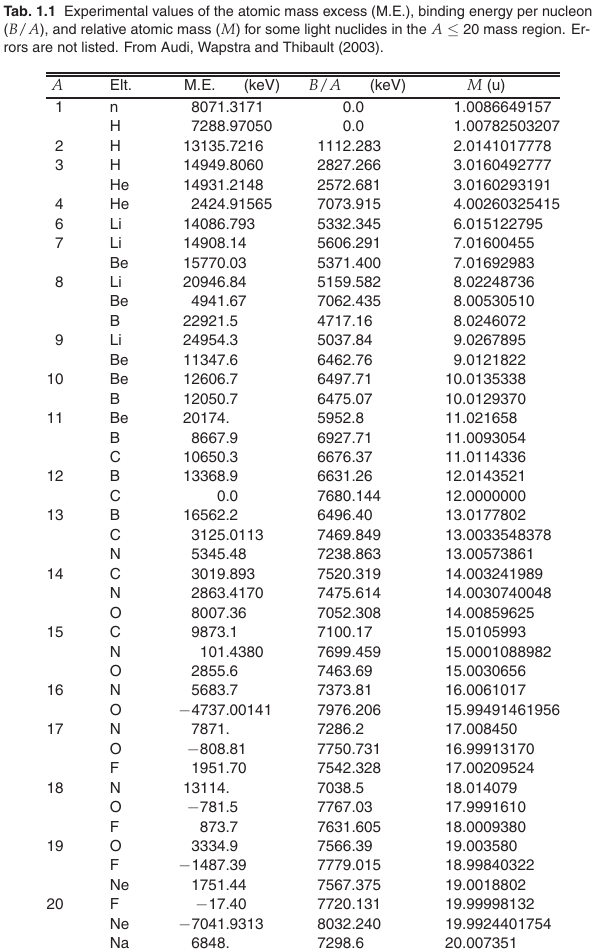
\includegraphics[trim={0.0cm 0cm 0.0cm 0},clip, keepaspectratio,height=0.9\textheight]{mass-excess}\label{fig:mass-excess}
			\end{figure}
        \end{column}
    \end{columns} 
\end{frame}

\begin{frame}{Binding Energies}
    \begin{columns}[T]
        \begin{column}{0.5\textwidth}
            \begin{align*}
                &m_uc^2=\SI{931.494}{\mega\ev}\\
                &m_{nuc}=Zm_p+Nm_n-\Delta m\\
                &B(Z,A)=(Zm_p+Nm_n-m_{nuc})c^2\\
                &2d\to\alpha:\\
                &\frac{B(d)}{A}=\SI{1.112}{\mega\ev},\frac{B(\alpha)}{A}=\SI{7.074}{\mega\ev}\\
                &Q=\SI{28.296}{\mega\ev}-\SI{2.224}{\mega\ev}-\SI{2.224}{\mega\ev}\\
                &=\SI{23.85}{\mega\ev}\tag{En. release}
            \end{align*}
        \end{column}
        \begin{column}{0.5\textwidth}
            \begin{figure}[!ht]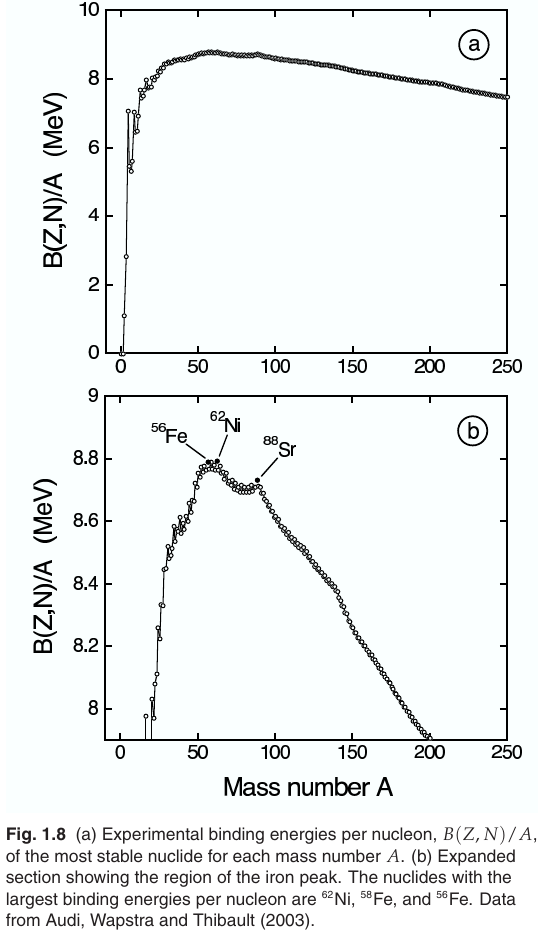
\includegraphics[trim={0.0cm 0cm 0.0cm 0},clip, keepaspectratio,height=0.9\textheight]{binding-energy}\label{fig:binding-energy}
			\end{figure}
        \end{column}
    \end{columns}
\end{frame}

\begin{frame}{Nuclear elastic scattering: \schr{} eq., partial waves}
    \begin{columns}[T]
        \begin{column}{0.55\textwidth}
            \begin{align*}
                &\psi=f(r)Y_l^m(\theta,\phi), L=\vecp{r}{p}=\frac{\hbar}{i}\vecp{r}{\nabla}\\
                &-\frac{\hbar^2}{2\mu}\nabla^2\psi+V(r)\psi=E\psi\\
                &-\frac{\hbar^2}{2\mu}=-\frac{\hbar^2}{2\mu}(\PtwoDof{r}+\frac{2}{r}\PDof{r})+\frac{L^2}{2\mu r^2}=\frac{p_r^2}{2\mu}+\frac{L^2}{2\mu r^2}\\
                &-\frac{\hbar^2}{2\mu}\TtwoDy{r}{\chi_l}+[\frac{l(l+1)\hbar^2}{2\mu r^2}+V(r)-E]\chi_l=0\tag{$f_l=\frac{\chi_l(r)}{r}$}\\
                &\psi(\vec{r})=N[\exp{i\scap{k}{r}}+f(\theta)\frac{\exp{ikr}}{r}]\tag{beam+target, $r\to\infty$}\\
                &\exp{i\scap{k}{r}}\to\exp{ikz}:u_l^{f.p.}=(kr)j_l(kr)\tag{free p.: Sol $j_l(kr)$ sph. Bessel}\\
                &\xrightarrow{\to\infty}\sin{(kr-\frac{l\pi}{2})},u_{l=0}^{f.p.}=\sin{(kr)}\\
                &\psi_T^{f.p.}=\exp{ikz}=\sum_{l=0}^{\infty}\underbrace{(2l+1)i^l}_{c_l}j_l(kr)P_l(\cos{\theta})\\
                &\xrightarrow{\to\infty}\frac{1}{2kr}\sum_{l=0}^{\infty}(2l+1)i^{l+1}[\exp{-i(kr-\frac{l\pi}{2})}-\exp{i(kr-\frac{l\pi}{2})}]P_l(\cos{\theta})\\
                &u_l=\sin{(kr-\frac{l\pi}{2}+\delta_l)}\tag{$r\to\infty$: $V=0$ same eq.}\\
                &\psi_T=\exp{ikz}+f(\theta)\frac{\exp{ikr}}{kr}\\
                &\xrightarrow{r\to\infty}\sum_{l=0}^{\infty}(2l+1)i^l\exp{i\delta_l}\frac{\sin{(kr-\frac{l\pi}{2}+\delta_l)}}{kr}P_l(\cos{\theta})\\
                &=\frac{1}{2kr}\sum_l^{\infty}(2l+1)i^{l+1}[\exp{-i(kr-\frac{l\pi}{2})}-\exp{2i\delta_l}\exp{i(kr-\frac{l\pi}{2})}]P_l(\cos{\theta})
            \end{align*}
        \end{column}
        \begin{column}{0.45\textwidth} 
            \begin{figure}[!ht]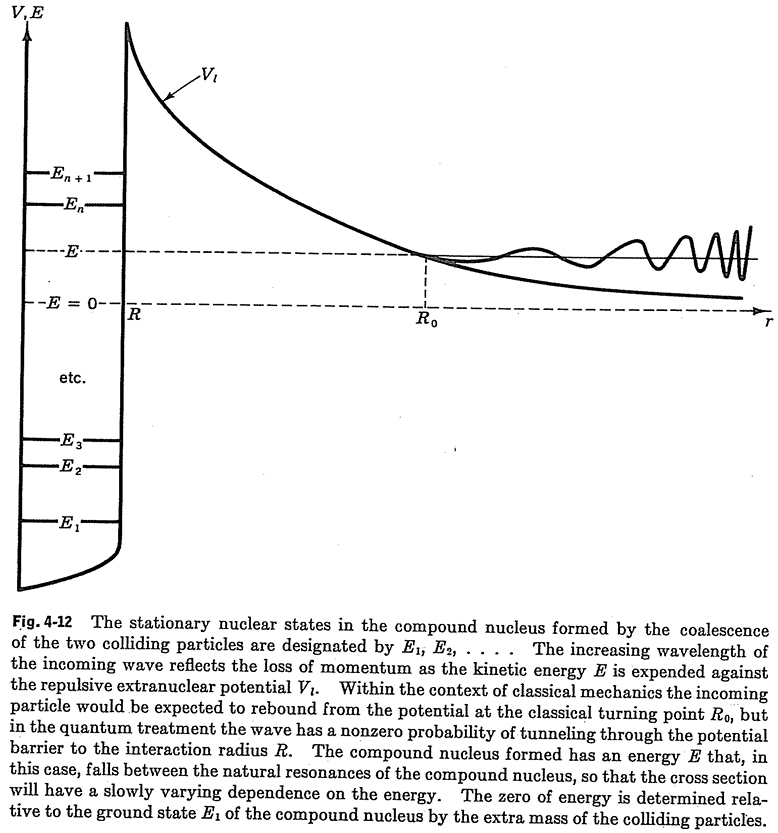
\includegraphics[trim={0.0cm 0cm 0.0cm 0},clip, keepaspectratio,width=0.9\textwidth]{nuclear-potential}\label{fig:nuclear-potential}
			\end{figure}
            \begin{align*}
                &R\approx1.4(A_1^{\frac{1}{3}}+A_2^{\frac{1}{3}})\SI{e-13}{\cm}\\
                &P=\psi^*\psi,j=vP\tag{particle-den, current-d.}\\
                &j_b=N^2v_b, j_s=v_sN^2|f(\theta)|^2 \frac{1}{r^2},dF=r^2d\Omega\\
                &\frac{N_e^{d\Omega}}{t}=\TDy{\sigma}{\Omega}\frac{N_b/t}{A}N_t\,d\Omega\tag{emitted}\\
                &\TDy{\sigma}{\Omega}=\frac{j_{et}\,dF}{j_b\,d\Omega}=\frac{j_sr^2}{j_b}=|f(\theta)|^2,j_{et}=\frac{N_{et}^{d\Omega}}{dF}
            \end{align*}
        \end{column}
    \end{columns}
\end{frame}

\begin{frame}{Elastic Scattering CrossSection}
    \begin{columns}[T]
        \begin{column}{0.7\textwidth}
            \begin{align*}
                &f(\theta)\frac{\exp{ikr}}{kr}=\psi_T-\psi_T^{f.p.}=\frac{1}{2kr}\sum_l(2l+1)i^{l+1}[\exp{i(kr-\frac{l\pi}{2})}(1-\exp{2i\delta_l})]P_l(\cos{\theta})\\
                &\exp{i \frac{\pi l}{2}}=\cos{\frac{\pi l}{2}}+i\sin{\frac{\pi l}{2}}=i^l, \exp{i\delta}\sin{\delta}=\frac{i}{2}(1-\exp{2i\delta}):\\
                &f(\theta)=\frac{1}{k}\sum_l(2l+1)\exp{i\delta_l}\sin{\delta_l}P_l(\cos{\theta})\\
                &(\TDy{\Omega}{\sigma})_{el}=f^*(\theta)f^*(\theta)=\frac{1}{k^2}|\sum_l(2l+1)\sin{\delta_l}P_l(\cos{\theta})|^2\\
                &\int_{d\Omega}P_l(\cos{\theta}P_{l'}(\cos{\theta}))\,d\Omega=\frac{4\pi}{2l+1}\delta_{ll'}:\\
                &\sigma_{el}=\sum_l\sigma_{el,l}=\sum_l \frac{\pi}{k^2}(2l+1)|1-\exp{2i\delta_l}|^2=\frac{4\pi}{k^2}(2l+1)\sin^2{\delta_l}
            \end{align*}
        \end{column}
        \begin{column}{0.3\textwidth}
        \end{column}
    \end{columns}
    \begin{columns}[T]
        \begin{column}{0.6\textwidth}
            \begin{align*}
                &(\TDy{\Omega}{\sigma})_{el,0}=\frac{1}{k^2}\sin^2{\delta_0},\sigma_{el,0}=\frac{4\pi}{k^2}\sin^2{\delta_0}\\
                &\delta_l\to\delta_l+\sigma_l:\tag{charged particles}\\
                &f(\theta)=\frac{i}{2k}\sum_l(2l+1)[1-\exp{2i(\delta_l+\sigma_l)}]P_l(\cos{\theta})\\
                &=\frac{i}{2k}\sum_l(2l+1)(1-\exp{2i\sigma_l})P_l(\cos{\theta})\tag{Rutherford s.}\\
                &+\frac{i}{2k}\sum_l(2l+1)\exp{2i\sigma_l}(1-\exp{2i\delta_l})P_l(\cos{\theta})\tag{N+C}
            \end{align*}
        \end{column}
        \begin{column}{0.4\textwidth}
            \begin{align*}
                &1-\exp{2i(\delta_l+\sigma_l)}\\
                &=(1-\exp{2i\sigma_l})+\exp{2i\sigma_l}(1-\exp{2i\delta_l})
            \end{align*}
        \end{column}
    \end{columns}
    
\end{frame}

\begin{frame}{Reaction CrossSection}
    \begin{columns}[T]
        \begin{column}{0.5\textwidth}
            \begin{align*}
                &\int_{\Omega}j_T\,d\Omega=0\tag{elastic}\\
                &\sigma_{re}=\frac{r^2}{j_b}\int j_T\,d\Omega\tag{non elastic: net current of particles}\\
                &j_b=\frac{\hbar}{2mi}[\exp{-ikz}(\exp{ikz}ik)-\exp{-ikz}(-ik)\exp{ikz}]=\frac{\hbar k}{m}\\
                &j_T=\frac{\hbar}{4mkr^2}[|\sum_l(2l+1)i^{l+1}\exp{\frac{il\pi}{2}}P_l(\cos{\theta})|^2\\
                &-|\sum_l(2l+1)i^{l+1}\exp{2i\delta_l}\exp{\frac{-il\pi}{2}}P_l{\cos{\theta}}|^2]\\
                &\sigma_{re,l}=\frac{\pi}{k^2}(2l+1)(1-|\exp{2i\delta_l}|^2)\geq0\\
                &|\exp{2i\delta_l}|^2=1\tag{If $\delta_l$ real: only elastic-sc}\\
                &\sigma_{el,l}^{max}=\frac{4\pi}{k^2}(2l+1), \sigma_{re,l}=0\tag{max elastic-c.s.}\\
                &\sigma_{re,l}^{max}=\sigma_{el,l}=\frac{\pi}{k^2}(2l+1)\tag{max reaction-c.s.}
            \end{align*}
        \end{column}
        \begin{column}{0.5\textwidth}
            \begin{itemize}
                \item  $\psi_T$ represents elastic scattering w.f.
                    \item $j=\frac{\hbar}{2mi}(\psi^*\TDy{r}{\psi}-\TDy{r}{\psi^*}\psi)$
                \end{itemize}
            \begin{figure}[!ht]
                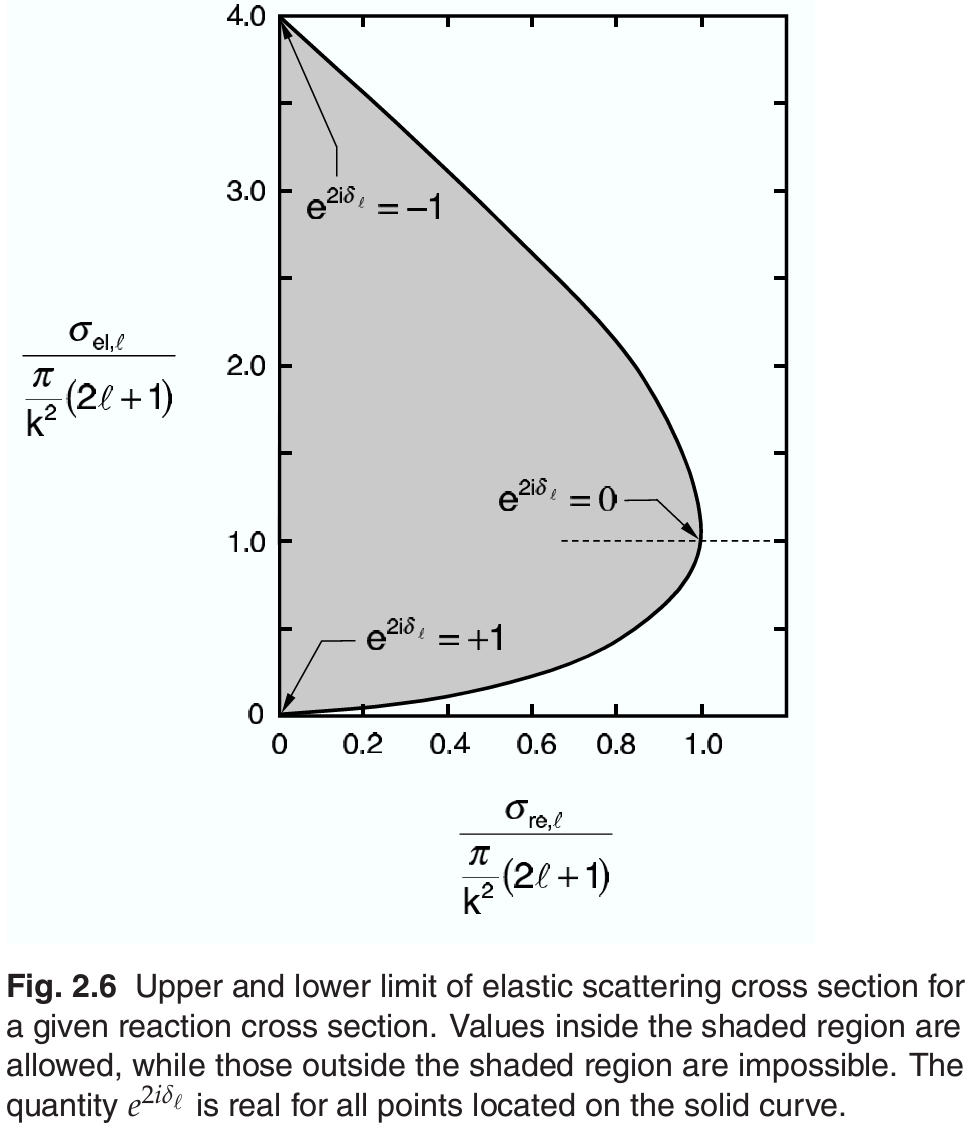
\includegraphics[trim={0.0cm 0cm 0.0cm 0},clip, keepaspectratio,width=0.9\textwidth]{scattering-reaction-cs}\label{fig:scattering-reaction-cs}
			\end{figure}
        \end{column}
    \end{columns}
\end{frame}

\begin{frame}{Transmission prob., phase shift and resonance phenomenon: T defined only in 1D}
    \begin{columns}[T]
        \begin{column}{0.75\textwidth}
        \begin{align*}
            &\TtwoDy{r}{u}+\frac{2m}{\hbar^2}[E-V(r)]u=0: \TtwoDy{r}{u}+\hat{k}u=0\tag{$l=0$, V const}\\
            &u=\alpha\exp{i\hat{k}r}+\beta\exp{-i\hat{k}r}, r<R_0: K^2=\frac{2m}{\hbar^2}(E+V_0), r>R_0: k^2=\frac{2m}{\hbar^2}E\\
            &u_{in}=A'\exp{iKr}B'\exp{-iKr}, u_{in}(0)=0=A'+B'\Rightarrow u_{in}=A\sin{(Kr)}\\
            &u_{out}=C'\exp{ikr}+D'\exp{-ikr}=\tag{$\sin{(x\pm y)}=\sin{x}\cos{y}\pm\cos{x}\sin{y}$}\\
            &C''\sin{(kr)}+D''\cos{(kr)}=C[\sin{(kr)}\cos{\delta_0}+\cos{(kr)}\sin{\delta_0}]=C\sin{(kr+\delta_0)}\\
            &\exp{-i\omega t}\tag{temporal evol: B' propagate negative x, C',D' reflected/moving toward $R_0$}\\
            &j_{tr}=v_{in}|B'|^2, j_{refl}=v_{out}|C'|^2,j_{inc}=v_{out}|D'|^2: T=\frac{j_{tr}}{j_{inc}}=\frac{v_{in}|B'|^2}{v_{out}|D'|^2}=\frac{K|B'|^2}{k|D'|^2}\\
            &\left.\begin{array}{l}&A'\exp{iKR_0}+B'\exp{-iKR_0}=C'\exp{ikR_0}+D'\exp{-ikR_0}\\&\frac{K}{k}(A'\exp{iKR_0}-B'\exp{-iKR_0})=(C'\exp{ikR_0}-D'\exp{-ikR_0})\\
            \end{array}\right\}
            \tag{cont cond}\\
            &\frac{K}{k}(-B'\exp{-iKR_0})=B'\exp{-iKR_0}-2D'\exp{-ikR_0}: \frac{B'}{D'}=2 \frac{\exp{-ikR_0}}{\exp{-iKR_0}}\frac{k}{k+K},A'=0\\
            &T=\frac{K|B'|^2}{k|D'|^2}=4 \frac{kK}{(k+K)^2}=4 \frac{\frac{2m}{\hbar^2}\sqrt{(E+V_0)E}}{[\sqrt{\frac{2m}{\hbar^2}(E+V_0)}+\sqrt{\frac{2m}{\hbar^2}E}]^2}\\
            &\left.\begin{array}{l}&A\sin{(KR_0)}=C\sin{(kR_0+\delta_0)}\\&AK\cos{(KR_0)}=Ck\cos{(kR_0+\delta_0)}\\
            \end{array}\right\}\Rightarrow \frac{1}{K}\tan{(KR_0)}=\frac{1}{k}\tan{(kR_0+\delta_0)}
        \end{align*}
        \end{column}
        \begin{column}{0.25\textwidth}
            \begin{figure}[!ht]
            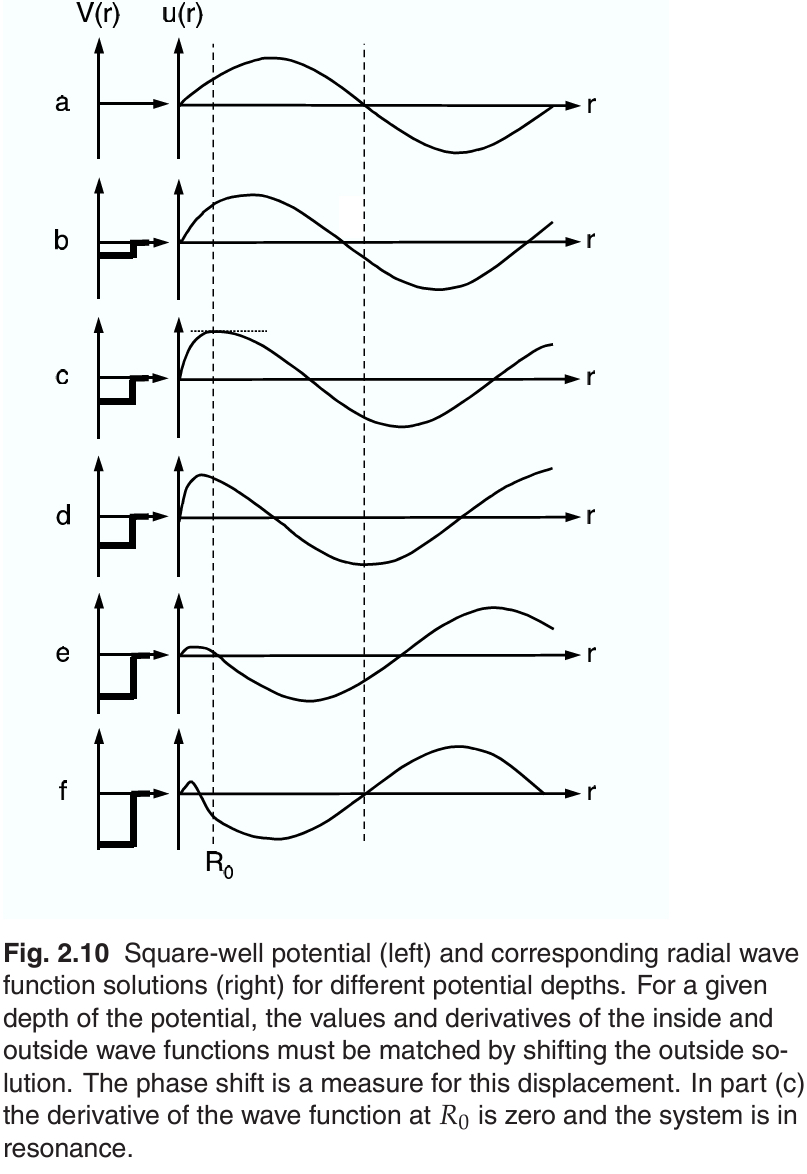
\includegraphics[trim={0.0cm 0cm 0.0cm 0},clip, keepaspectratio,width=0.8\textwidth]{pot-shift}\label{fig:pot-shift}
			\end{figure}
        \end{column}
    \end{columns}
    \begin{align*}
        &\delta_0=-kR_0+\arctan{[\frac{k}{K}\tan{(KR_0)}]}=-\frac{\sqrt{2mE}}{\hbar}R_0+\arctan{[\sqrt{\frac{E}{E*V_0}}\tan{(\frac{\sqrt{2m(E+V_0)}}{\hbar}R_0)}]}\\
        &
    \end{align*}
\end{frame}

\begin{frame}{Resonances}
    Squarin and addin continuity conditions:
    \begin{columns}[T]
        \begin{column}{0.6\textwidth}
        \begin{align*}
            &\frac{|A|^2}{|C|^2}=\frac{k^2}{k^2+[K^2-k^2]\cos^2{(KR_0)}}=\frac{E}{E+V_0\cos^2{(\frac{\sqrt{2m(E+V_0)}}{\hbar}R_0)}}\\
            &\cos^2{KR_0}=0: KR_0=(n+\frac{1}{2})\pi: K=\frac{(n+\frac{1}{2})\pi}{R_0}=\frac{2\pi}{\lambda_{in}}\\
            &\lambda_{in}=\frac{2R_0}{(n+\frac{1}{2})}=\frac{R_0}{(\frac{n}{2}+\frac{1}{4})}\tag{$\lambda_{in}$ wavelength in interior}\\
            &E_n=\frac{\hbar^2}{2m}\frac{\pi^2}{R_0^2}(n+\frac{1}{2})^2-V_0\tag{resonance energy: $\frac{n}{2}+\frac{1}{4}$ wavelength fit into interior}
        \end{align*}
        \begin{columns}[T]
            \begin{column}{0.45\textwidth}
            \begin{figure}[!ht]
            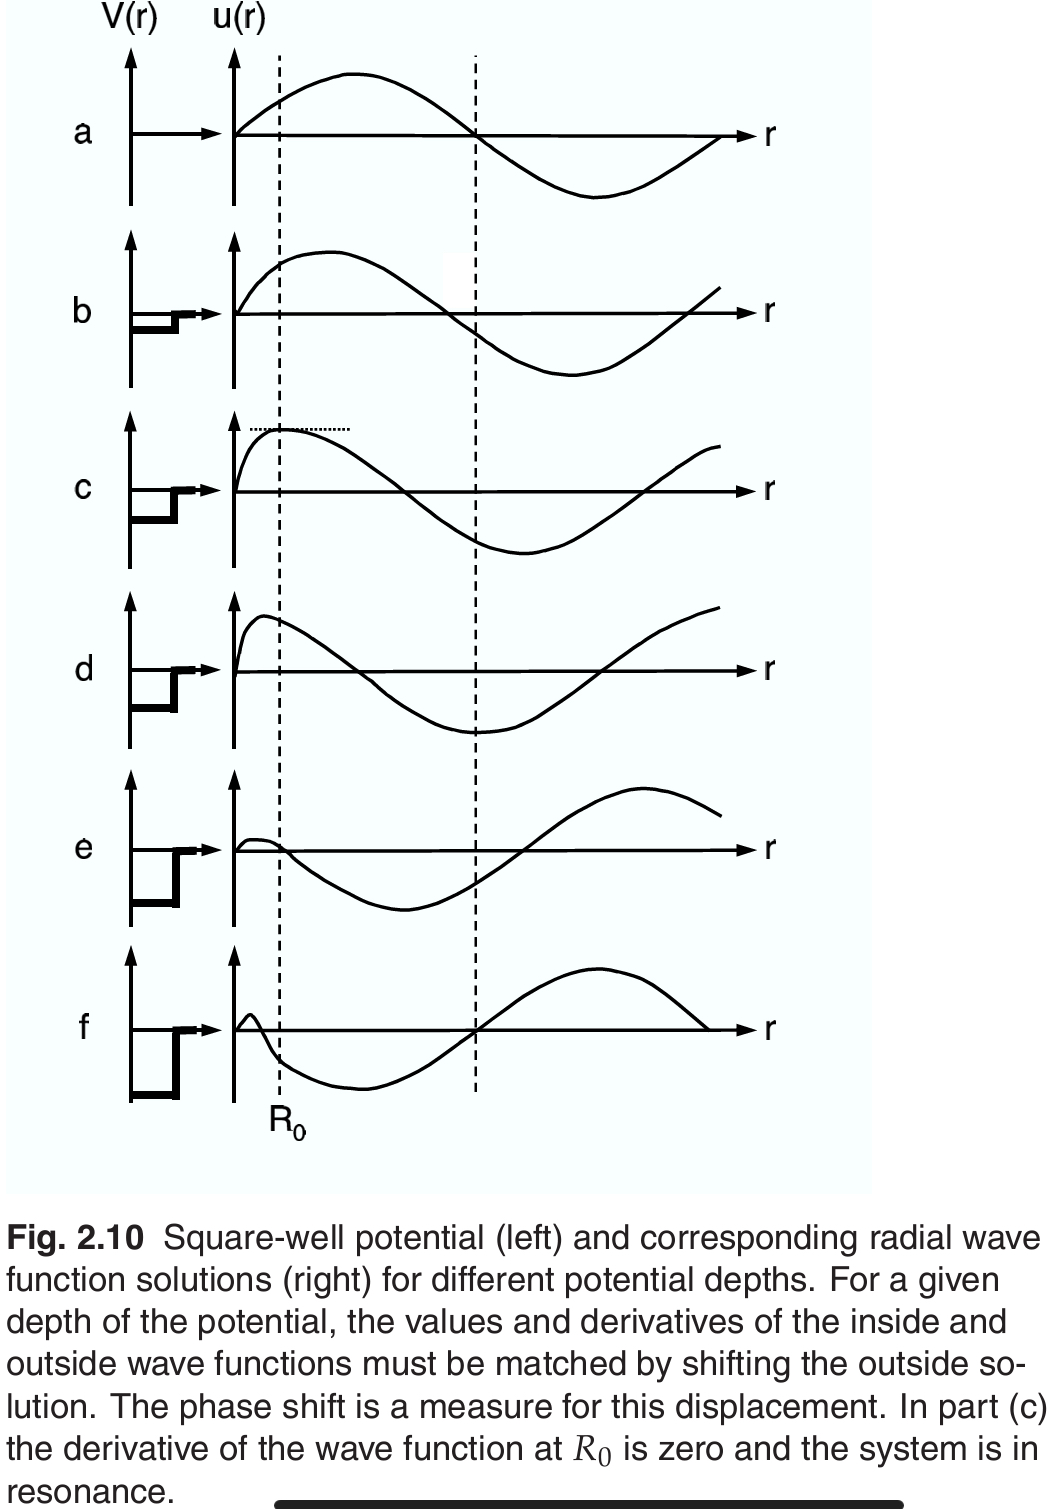
\includegraphics[trim={0.0cm 0cm 0.0cm 0},clip, keepaspectratio,width=0.9\textwidth]{wavefunction-phaseshift}\label{fig:wavefunction-phaseshift}
			\end{figure}
            \end{column}
            \begin{column}{0.55\textwidth}
            \end{column}
        \end{columns}
    \end{column}
        \begin{column}{0.4\textwidth}
            \begin{figure}[!ht]
            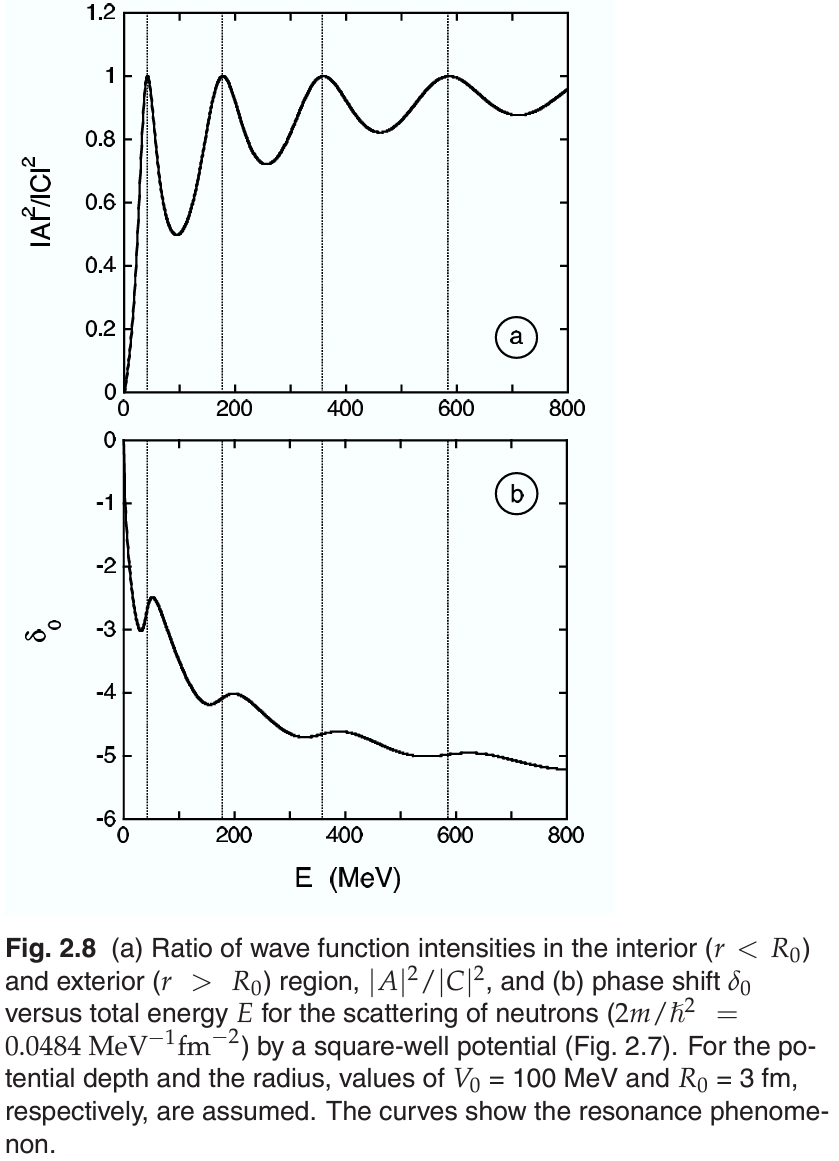
\includegraphics[trim={0.0cm 0cm 0.0cm 0},clip, keepaspectratio,width=0.9\textwidth]{phaseshift-res}\label{fig:phaseshift-res}
			\end{figure}
            At resonance energies $E_i$ prob finding particle inside $r<R_0$ is at maximum; each res shift phase $\delta_0$ by some amount
        \end{column}
    \end{columns}
\end{frame}

\begin{frame}{Resonance in square barrier potential}
                \begin{align*}
                    &u_I=A'\sin{(Kr)},u_{II}=C\exp{-\kappa r}+D\exp{\kappa r}, u_{III}=F'\sin{(kr+\delta_0')},\Delta=R_1-R_0\\
                    &\delta_0=-kR_1+\arctan{[\frac{k}{\kappa}\frac{\sin{(KR_0)}(\exp{-\kappa\Delta}+\exp{\kappa\Delta})+\frac{K}{\kappa}\cos{(KR_0)}(\exp{\kappa\Delta}-\exp{-\kappa\Delta})}{\sin{(KR_0)}(\exp{\kappa\Delta}-\exp{-\kappa\Delta})+\frac{K}{\kappa}\cos{(KR_0)}(\exp{-\kappa\Delta}-\exp{\kappa\Delta})}]}\\
                    &\frac{|F'|^2}{|A'|^2}=\sin^2{KR_0}+(\frac{K}{k})^2\cos^2{(KR_0)}+\sin^2{(KR_0)}\sinh^2{(\kappa\Delta)}[1+(\frac{\kappa}{k})^2]+\cos^2{(KR_0)}\sinh^2{(\kappa\Delta)}[(\frac{K}{\kappa})^2\\
                    &+(\frac{K}{k})^2]+\sin{(KR_0)}\cos{(KR_0)}\sinh{(2\kappa\Delta)}[(\frac{K}{\kappa})+(\frac{K}{\kappa})(\frac{\kappa}{k}^2)]
                \end{align*}
    \begin{columns}[T]
        \begin{column}{0.33\textwidth}
            \begin{figure}[!ht]
            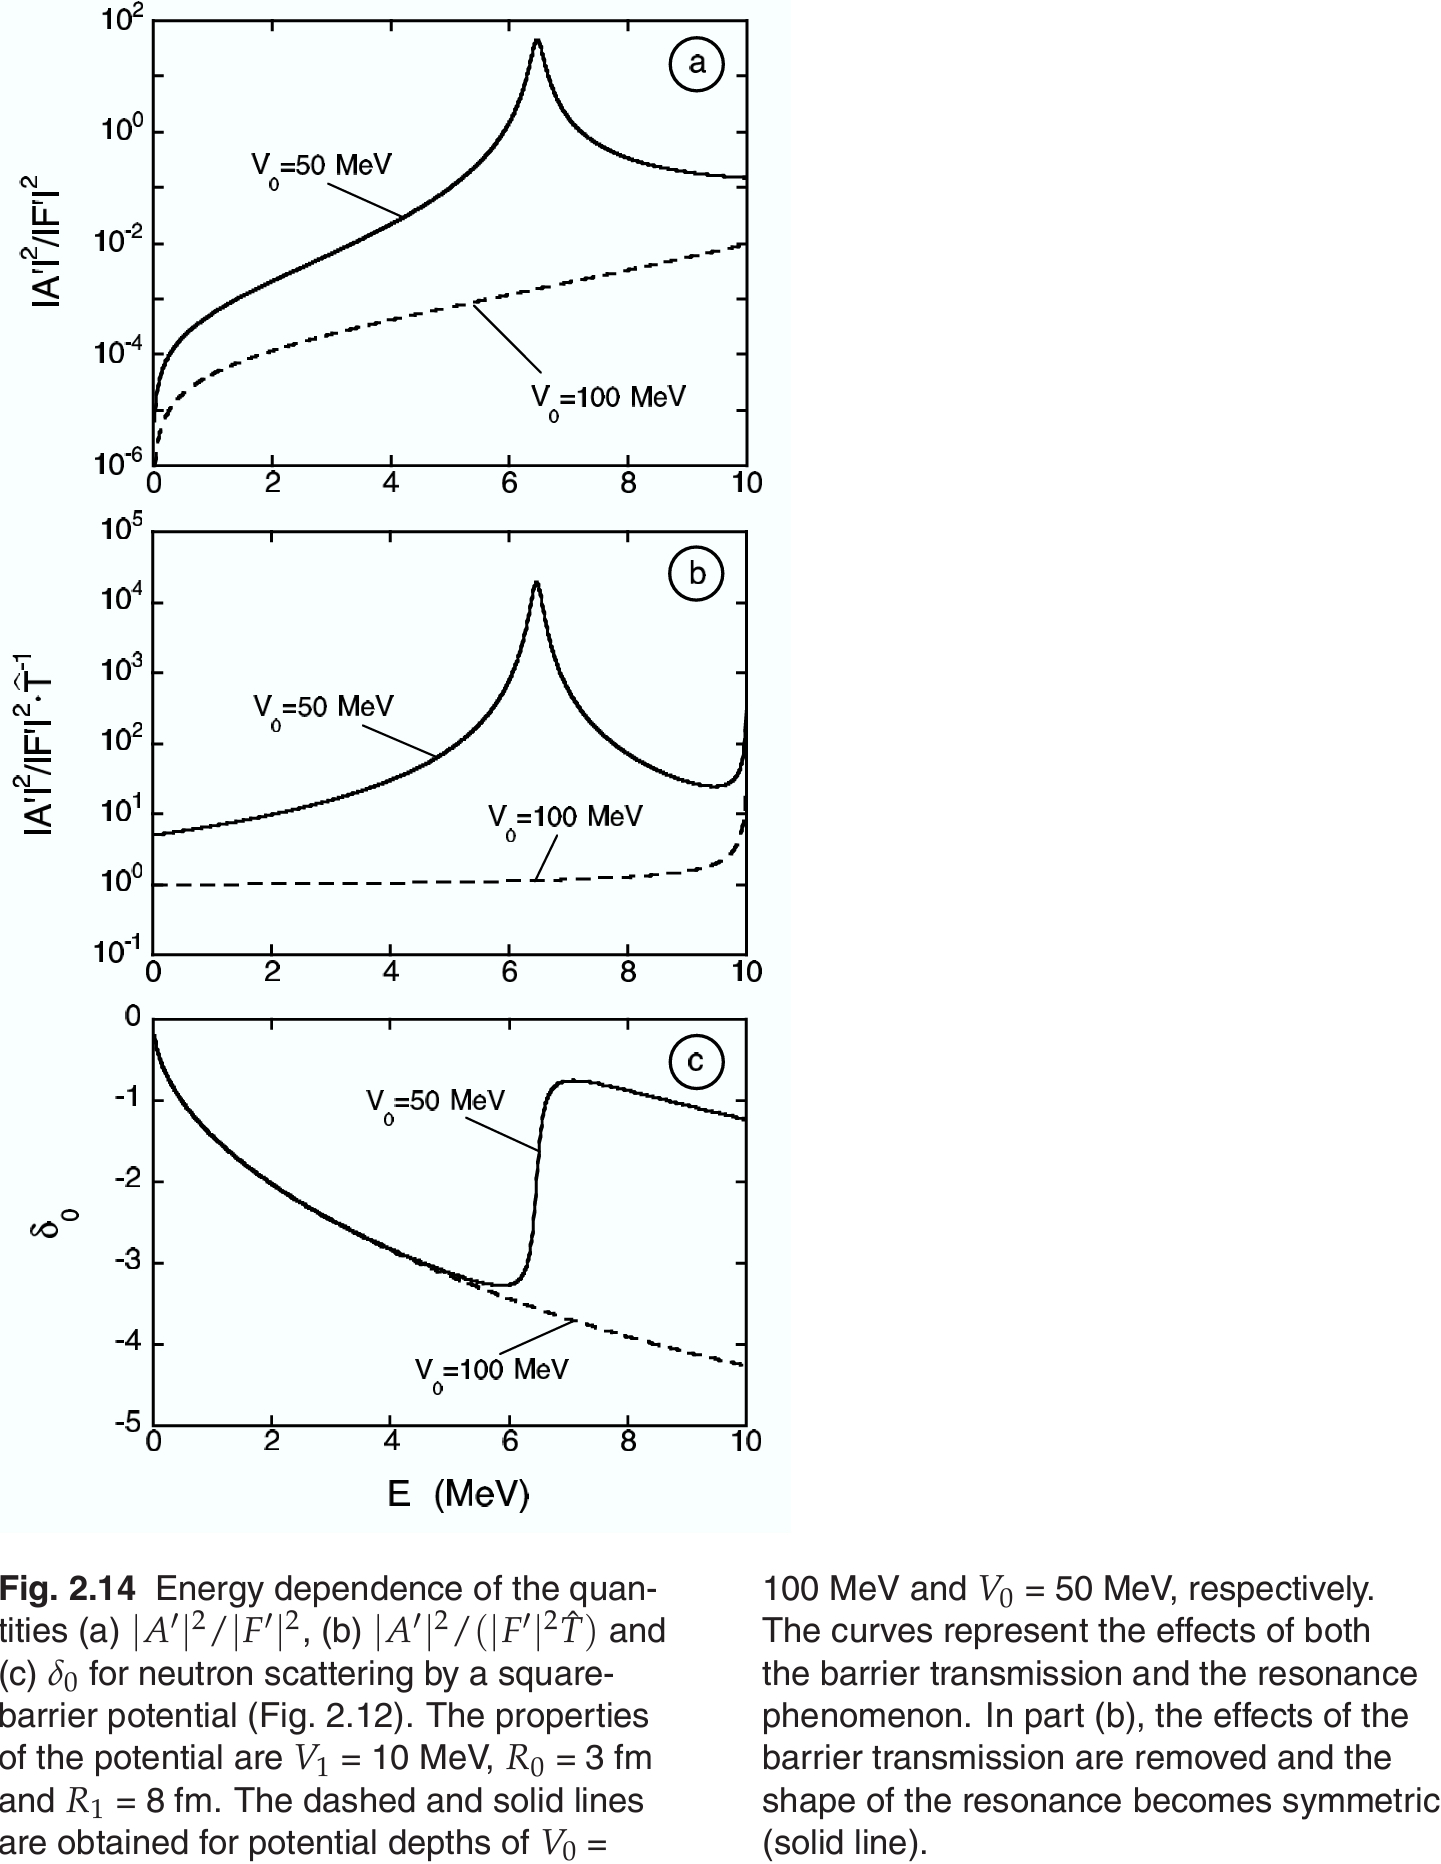
\includegraphics[trim={0.0cm 0cm 0.0cm 0},clip, keepaspectratio,width=0.9\textwidth]{resonance-squarebarrier}\label{fig:resonance-squarebarrier}
			\end{figure}
        \end{column}
        \begin{column}{0.33\textwidth}
            \begin{figure}[!ht]
            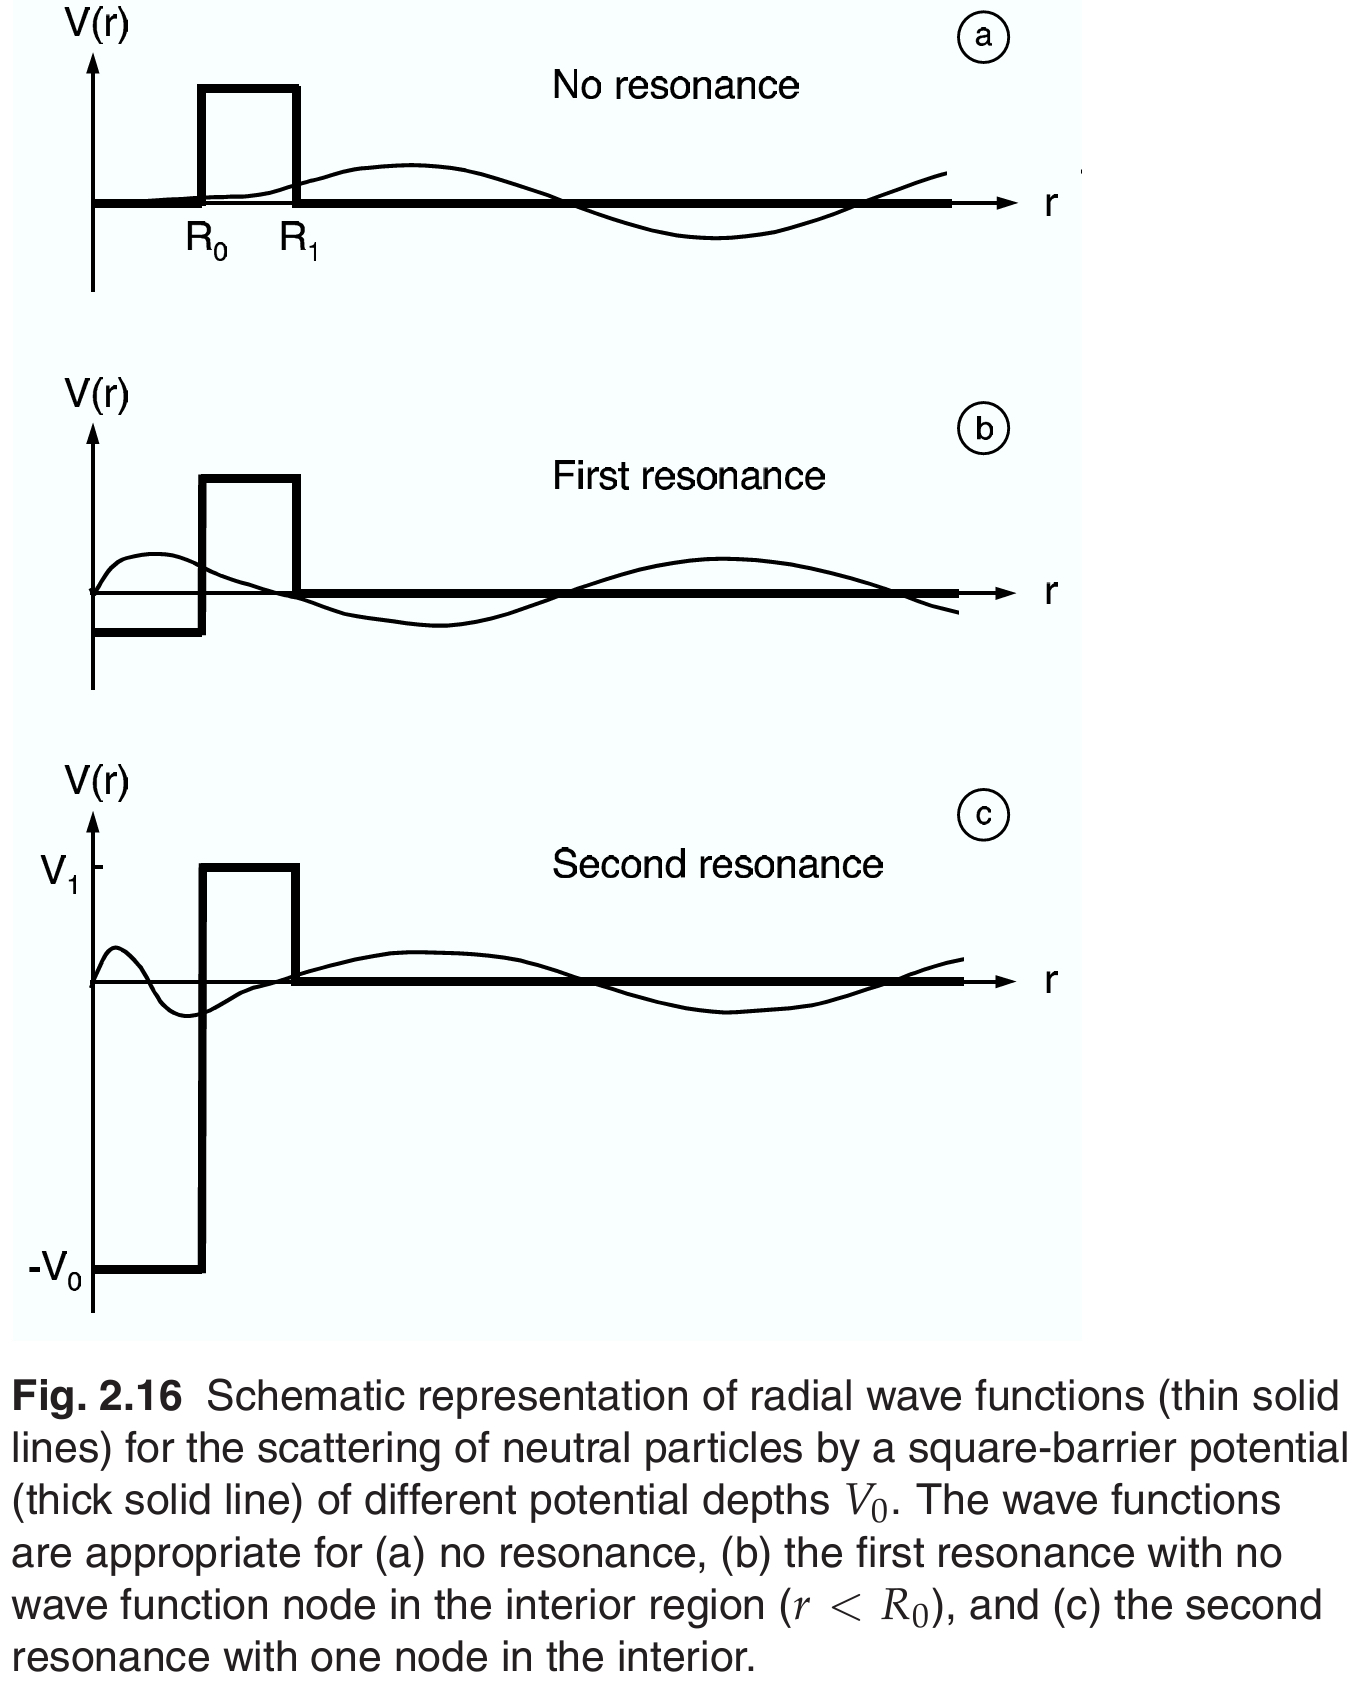
\includegraphics[trim={0.0cm 0cm 0.0cm 0},clip, keepaspectratio,width=0.9\textwidth]{wavefunction-resonance-barrier}\label{fig:wavefunction-resonance-barrier}
			\end{figure}
        \end{column}
        \begin{column}{0.33\textwidth}
            \begin{figure}[!ht]
            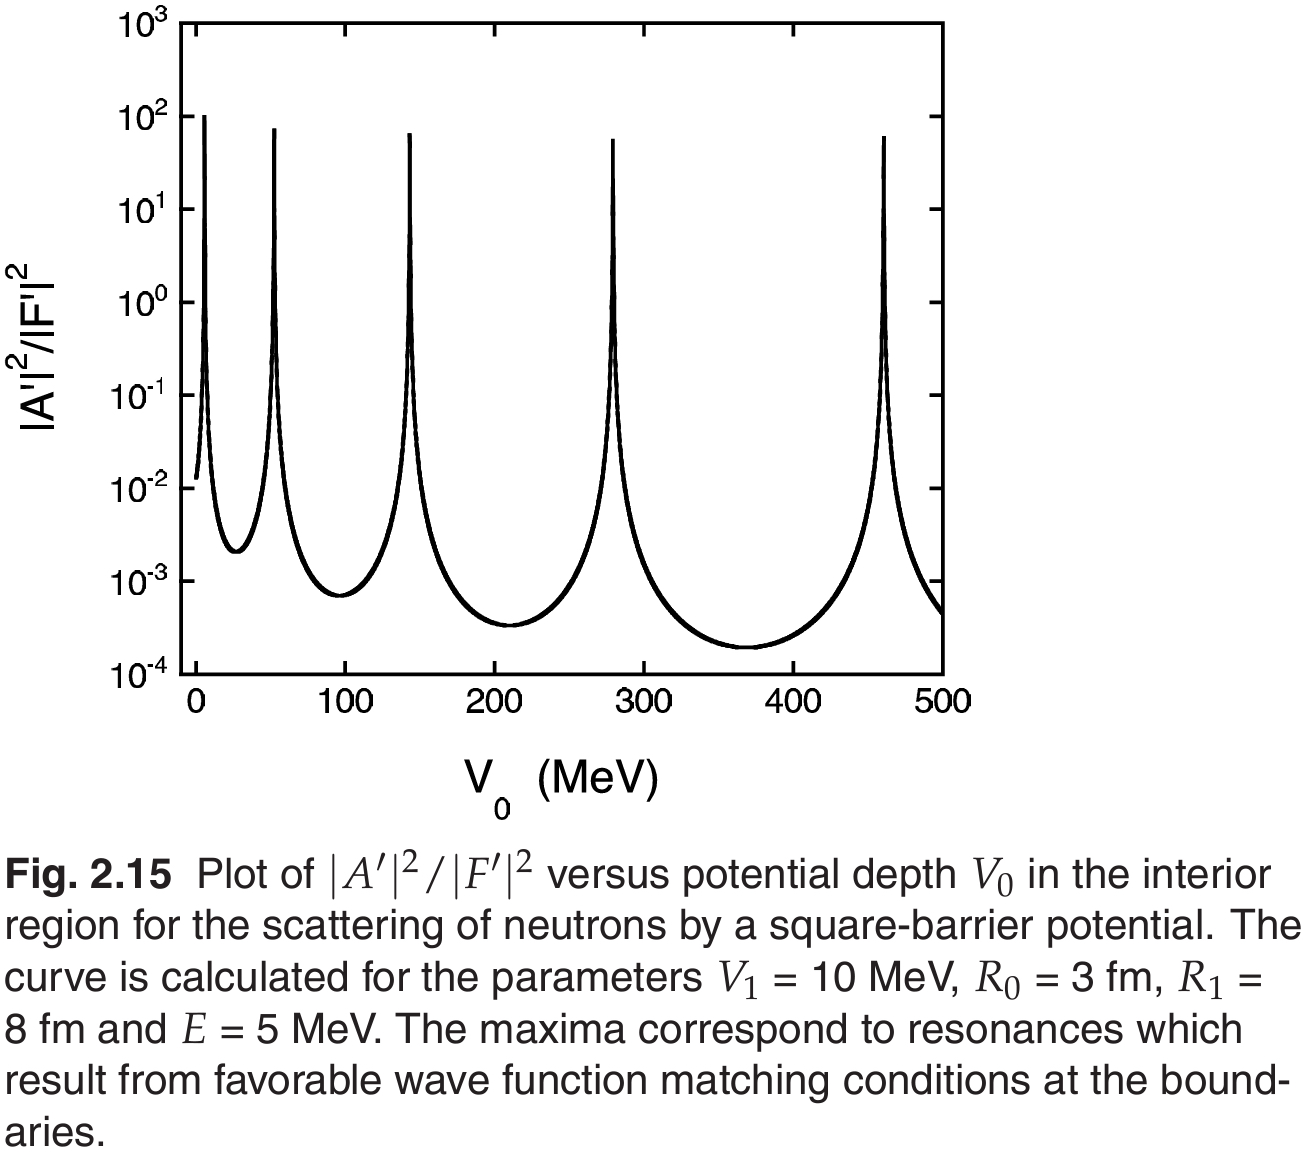
\includegraphics[trim={0.0cm 0cm 0.0cm 0},clip, keepaspectratio,width=0.9\textwidth]{A2_F2-barrier}\label{fig:A2_F2-barrier}
			\end{figure}
        \end{column}
    \end{columns}
\end{frame}

\begin{frame}{Scattering: square barrier potential transmission (1D)}
    \begin{columns}[T]
        \begin{column}{0.7\textwidth}
            \begin{align*}
                &(u_I)_{R_0}=(u_{II})_{R_0}, (\TDy{x}{u_I})_{R_0}=(\TDy{x}{u_{II}})_{R_0}\\
                &(u_{II})_{R_1}=(u_{III})_{R_1}, (\TDy{x}{u_{II}})_{R_1}=(\TDy{x}{u_{III}})_{R_1}\\
                &A\alpha\exp{iKR_0}+B\alpha^*\exp{-iKR_0}=\exp{-\kappa(R_1-R_0)}(F\beta\exp{ikR_1}+G\beta^*\exp{-ikR_1})\\
                &A\alpha^*\exp{iKR_0}+B\alpha\exp{-iKR_0}=\exp{\kappa(R_1-R_0)}(F\beta^*\exp{ikR_1}+G\beta\exp{-ikR_1})\\
                &\alpha=1+i \frac{K}{\kappa}, \beta=1+i\frac{k}{\kappa}, \Delta=R_1-R_0\\
                &B[\alpha^*\beta^*\exp{\kappa\Delta}-\alpha\beta\exp{-\kappa\Delta}]=G[(\beta^*)^2-\beta^2]\exp{-i(kR_1-KR_0)}=-2i \frac{k}{\kappa}G\exp{-i(kR_1-KR_0)}\\
                &T=\frac{K|B|^2}{k|G|^2}=\frac{4Kk/\kappa^2}{|\alpha^*\beta^*\exp{\kappa\Delta}-\alpha\beta\exp{-\kappa\Delta}|^2}\\
                &=\frac{Kk}{(k+K)^2+(\kappa^2+K^2+k^2+K^2k^2/\kappa^2)\sinh^2{\kappa\Delta}}\\
                &\frac{1}{T}=\frac{1}{\sqrt{E(E+V_0)}}[(2E+V_0+2 \sqrt{E(E+V_0)})+\\
                &+(E+V_0+V_1+\frac{E(E+V_0)}{V_1-E})\sinh^2{(\sqrt{\frac{2m}{\hbar^2}(V_1-E)}\Delta)}]\\
                &\kappa\Delta=\frac{\sqrt{2m(V_1-E)}}{\hbar}(R_1-R_0)\gg1\tag{low bombarding E/Thick barrier}\\
                &|\alpha^*\beta^*\exp{\kappa\Delta}-\alpha\beta\exp{-\kappa\Delta}|^2\approx|\alpha^*\beta^*\exp{\kappa\Delta}|^2\Rightarrow T\approx4 \frac{\sqrt{E(E+V_0)}(V_1-E)}{V_1(V_0+V_1)}\exp{-2\kappa(R_1-R_0)}\\
                &T\approx\exp{-\frac{2}{\hbar}\sqrt{2m(V_1-E)}(R_1-R_0)}\tag{Strict: neutral, $l=0$ scatt.}
            \end{align*}
        \end{column}
        \begin{column}{0.25\textwidth}
            \begin{figure}[!ht]
                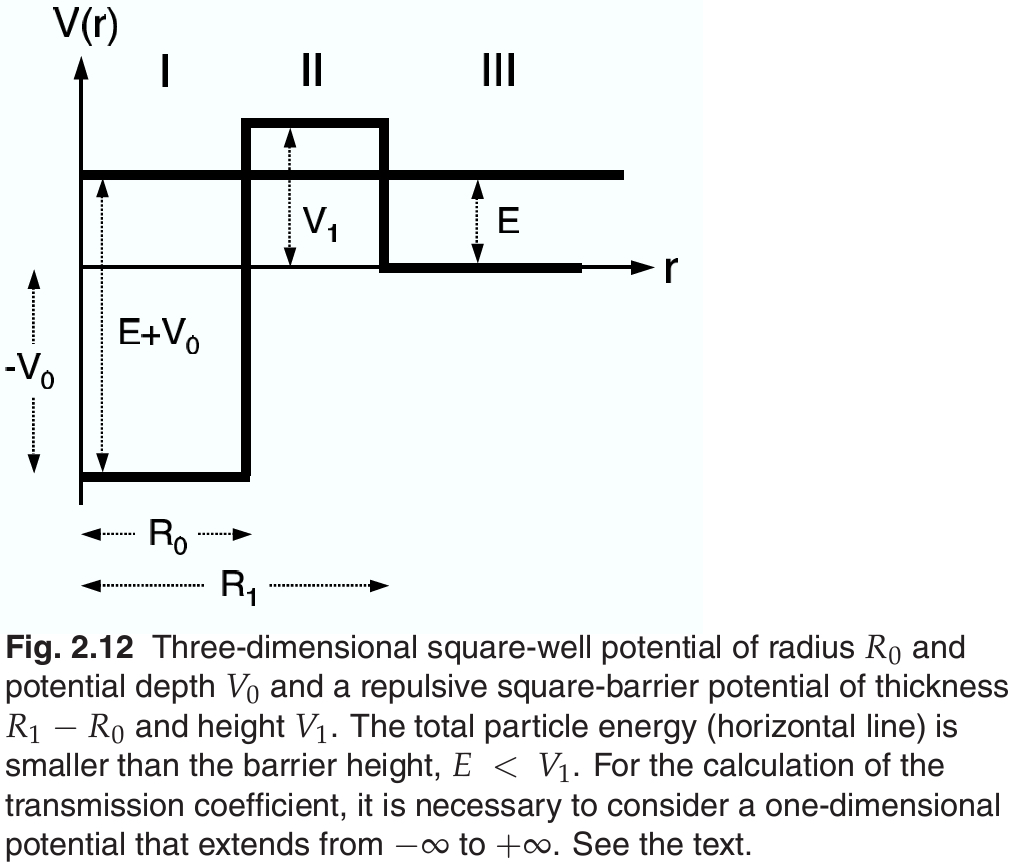
\includegraphics[trim={0.0cm 0cm 0.0cm 0},clip, keepaspectratio,width=0.8\textwidth]{nuclear-square-barrier}\label{fig:nuclear-square-barrier}
                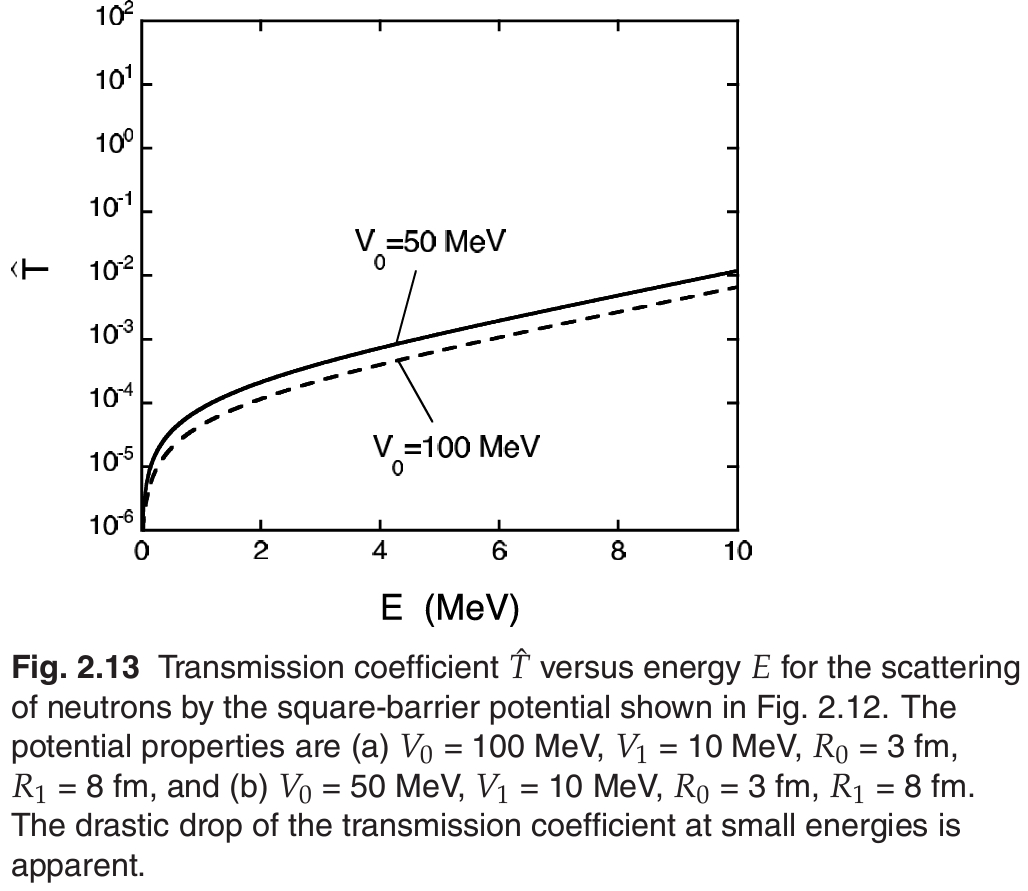
\includegraphics[trim={0.0cm 0cm 0.0cm 0},clip, keepaspectratio,width=0.8\textwidth]{transcoeff-squarebarrier}\label{fig:transcoeff-squarebarrier}
			\end{figure}
            1D radial wave-function:
            \begin{align*}
                &u_I=A\exp{iKx}+B\exp{-iKx}\\
                &u_{II}=C\exp{-\kappa x}+D\exp{\kappa x}\\
                &u_{III}=F\exp{ikx}+G\exp{-ikx}\\
                &T=\frac{j_{trans}}{j_{inc}}=\frac{K|B|^2}{k|G|^2}\\
                &A=0\tag{no wave from left}\\
                &F=0
            \end{align*}
        \end{column}
    \end{columns}
    
\end{frame}

\subsection{Stellar model}

\subsection{stars formation}

\subsection{Model computation}

\subsection{Sun model and helioseism}

\subsection{Composition: initial params and evolution}

\begin{frame}{programma per questa sezione}
    \begin{itemize}
        \item Def Z etc composizione solare, BBN: 210216
        \item Structural deps on composition: 20210315
        \item Composizione e opacit\'a/T: 20210326, 20210329, 20210330, 20210426
        \item CNO burning
        \item processi s
        \item produzione elementi pesanti:20210420
        \item Zams: variazione con comp: 20210503
        \item Helium to metal enrichment $\frac{\Delta Y}{\Delta Z}$, broadening observed MS
        \item Dredge-up: 20210507
        \item diffusione: 20210507
        \item Deps tip rgb on comp: 20210512
        \item Deps on chem of vertical/horizontal method: 20210517
        \item R param deps on Y: 20210521
        \item DredgeUpII: 20210521
        \item DredgeUpIII: 20210524
    \end{itemize}
\end{frame}

\subsection{Polytropic}

\subsection{Homologous stars}

\begin{frame}{H.models}
\begin{itemize}
    \item  Homologus star:they have the same $\frac{T}{T_c}$, $\frac{P}{P_c}$, $\frac{\rho}{\rho_c}$ when expressed in terms of $\frac{r}{R}$.
\end{itemize}
    
\end{frame}

\subsection{Grandezze Fondamentali}\linkdest{succo}

\begin{frame}{Stime Euristiche: Tempo scala, Pressione e Temperatura centrali}
    \begin{columns}[T]
        \begin{column}{0.5\textwidth}
            \begin{align*}
                &\PDy{m}{P}=-\frac{Gm}{4\pi r^4}\Rightarrow \frac{P_0-P_c}{M}\approx \frac{2G(M/2)^2}{4\pi(R/2)^4}\\
                &\Rightarrow P_c\approx \frac{2GM^2}{\pi R^4}\\
                &\rho\xrightarrow{\text{ideal g.}}\frac{\mu}{R}\frac{P}{T}\Rightarrow T_c\approx \frac{P_c}{\rho_c}\frac{\mu}{R}\\
                &=P_c\frac{\mu}{R}\underbrace{\frac{\bar{\rho}}{\rho_c}}_{\approx0.01-0.03}\Rightarrow T_c<\frac{8}{3}\frac{G\mu}{R}\frac{M}{R}
            \end{align*}
        \end{column}
        \begin{column}{0.5\textwidth}
            \begin{align*}
                &f_P=-\PDy{m}{P}\,dm\\
                &f_g=-\frac{g\,dm}{4\pi r^2}=-\frac{Gm}{r^2}\frac{dm}{4\pi r^2}\\
                &\frac{dm}{4\pi r^2}\PtwoDy{t}{r}=f_P+f_g\Rightarrow \frac{1}{4\pi r^2}\PtwoDy{t}{r}=-\PDy{m}{P}-\frac{Gm}{4\pi r^4}\\
                &|\PtwoDy{t}{r}|\to \frac{R}{\tau_{ff}}\Rightarrow \frac{R}{\tau_{ff}}\approx g\Rightarrow\tau_{ff}\approx\sqrt{\frac{R}{g}}\\
                &\to \frac{R}{\tau_{expl}^2}\Rightarrow \frac{R}{\tau_{expl}^2}=\frac{P}{\rho R}=4\pi r^2\PDy{m}{P}=\PDy{m}{P}/\rho\\
                &\Rightarrow\tau_{expl}\approx R\sqrt{\frac{\rho}{P}}
            \end{align*}
        \end{column}
    \end{columns}
R\end{frame}

\begin{frame}{Masse limite}
    \begin{itemize}
        \item $M_{up}$: Highest *-mass at which \Pelectron-degeneracy prevent C-ignition in CO core. Depends strongly on chem. composition - $M_{up}\approx8\msun{}$ at solar metallicity.
    \end{itemize}
\end{frame}

\subsection{Equazioni struttura: Energy transport}

\begin{frame}{Radiative transport}
    \begin{columns}[T]
        \begin{column}{0.5\textwidth}
            \begin{align*}
                &I(\theta)\,d\Omega=cu(\theta)\,d\Omega\\
                &u=\int^{4\pi}u(\theta)\,d\Omega=\frac{1}{c}\int I(\theta)\,d\Omega\tag{Energy density}\\
                &J(\vec{r},\nu,t)=\invers{(4\pi)}\int I(\vec{r},\hat{n},\nu,t)\,d\Omega\tag{Mean Intensity}\\
                &P_r=\frac{1}{3}\int_0^{\infty}\frac{h\nu}{c}cn(\nu)\,d\nu=\frac{1}{3}u\tag{rad Press}\\
                &P_r=\frac{1}{c}\int I(\theta)\cos^2{\theta}\,d\Omega\tag{Rad Press}\\
                &=\int^{4\pi}\frac{I(\theta)\cos{\theta}}{c}\cos{\theta}\,d\Omega\\
                &=\frac{2\pi}{c}\int_0^{2\pi}I(\theta)\cos{\theta}\sin{\theta}\,d\theta\\
                &H=\int I(\theta)\cos{\theta}\,d\Omega\\
                &=2\pi\int_0^{\pi}I(\theta)\cos{\theta}\sin{\theta}\,d\theta\tag{Net En. Flux polar dir}
            \end{align*}
        \end{column}
        \begin{column}{0.4\textwidth}
            Pressione di radiazione: radiazione contenuta in parallelepipedo di superficie unitaria lunghezza c in direzione $\theta$ (l'asse polare forma con la radiazione un angolo $\theta$) quindi la sezione d'urto geometrica in direzione polare contiene fattore $\cos{\theta}$, la proiezione del momento rispetto alla direzione polare ha un altro $\cos{\theta}$.
        \end{column}
    \end{columns}
\end{frame}

\begin{frame}{Flusso di energia proporzionale al gradiente termico}
\begin{block}{Diffusion Approx: Stellar Interior Near TE}
    \begin{columns}[T]
        \begin{column}{0.5\textwidth}
    \begin{align*}
                &U=aT^4\\
                &''\vec{j}=-D\nabla n''\tag{diffusion}\\
                &D=\frac{1}{3}vl_p\\
                &\vec{F}_{\nu}=-D_{\nu}\nabla U_{\nu}\\
                &D_{\nu}=\frac{1}{3}cl_{\nu}=\frac{c}{3\kappa_{\nu}}\rho
            \end{align*}
        \end{column}
        \begin{column}{0.5\textwidth}
            \begin{align*}
                &I(\theta)=I_0+I_1\cos{\theta}+\ldots\\
                &u=\frac{4\pi}{c}I_0\\
                &H=\frac{4\pi}{3}I_1\\
                &P_r=\frac{4\pi}{3c}I_0
            \end{align*}
        \end{column}
    \end{columns}
    
\end{block}

\begin{block}{Momentum transfer Rad-Mat}
    \begin{columns}[T]
        \begin{column}{0.6\textwidth}
    \begin{align*}
        &dp=\frac{dF_{Rad}}{c}=\frac{F_{Rad}}{c}\frac{dr}{l}\\
        &\TDy{r}{P_{Rad}}=-\frac{\kappa\rho}{c}F_{Rad}\\
        &-\frac{F_{rad}(\nu)}{c}\kappa_{\nu}\rho\,dr=\frac{4\pi}{3c}\TDy{r}{B_{\nu}(T)}\,dr\tag{L-grad T}
    \end{align*}
        \end{column}
        \begin{column}{0.4\textwidth}
            Flux of photons through volume matter at r, flux of energy $F_{rad}$. $dp$ momentum transfered from photons to volume element, $l$ photon mean free path: $\invers{l}=\kappa\rho$, $dp$ opposite of change of $dP_{Rad}$ of pressure exerted by photons over dr    
        \end{column}
    \end{columns}
    
\end{block}
\end{frame}

\subsection{evolution}

\begin{frame}{Pre-MS}
    \begin{itemize}
        \item Lithium but not berylium burn s at bottom of convective zone for less massive yhen $1.3\msun{}$.
    \end{itemize}
\end{frame}

\subsection{Equazioni da ricordare}

\begin{frame}{Pressione di radiazione}
Tutte le volte che un atomo emette/assorbe un fotone perde/guadagna quantit\'a di moto e dato che un atomo emette in maniera isotropa il momento netto \'e nullo una volta mediato su molte emissioni.
I processi di assorbimento non sono isotropicamente distribuiti dato il flusso uscente di energia per $cm^2$ per sec F: solo una frazione $\kappa$ del flusso di momento $\frac{F}{c}$ \'e assorbita dalla materia. Il trasferimento da parte della radiazione di momento alla materia per $cm^3$ per sec, cio\'e la forza esercitata dalla radiazione \'e $\kappa H \frac{1}{c}$.
Un elemento di volume $dS\,dr$ subisce per effetto dell'assorbimento della radiazione una variazione d'impulso $dq$, nel caso un fotone venga assorbito la variazione del flusso uscente \'e $dF<0$.
The distribution of photons over over different quantum states with energies $\epsilon_k=\hbar\omega_k$ (large volume $\omega_k\to\omega$)
\begin{align*}
\overline{n_k}=\frac{1}{\exp{\frac{\hbar\omega}{KT}}-1}
\end{align*}
Moltiplicando il numero di stati nel dato range di frequenze per la distribuzione di Plank (numero di occupazione) ottengo il numero di fotoni e l'energia radiativa nel range di frequenza
\begin{align*}
&dN_{\omega}=\frac{V}{\pi^2c^3}\frac{\omega^2\,d\omega}{\exp{\frac{\hbar\omega}{KT}}-1}\\
&dE_{\omega}=\frac{V\hbar}{\pi^2c^3}\frac{\omega^3\,d\omega}{\exp{\frac{\hbar\omega}{KT}}-1}
\end{align*}
\end{frame}

\begin{frame}{Gradiente per trasporto radiativo nell'interno stellare}
\begin{align*}
&dq=-(n_{\nu}\,dSc\,dt)*(\kappa\rho\,dr)*\frac{h\nu}{c}&\intertext{Il primo termine \'e il numero di fotoni pasanti per superficie $dS$ in tempo $dt$, il secondo \'e la probabilit\'a d'assorbimento attraverso spessore $dr$, il terzo \'e la quantit\'a di moto di ogni fotone.}\\
&dP_r=\TDy{S}{F}=\TDof{S}\TDy{t}{q}\\
&=-\int \,d\nu n_{\nu}c\kappa_{\nu}\rho\,dr\frac{h\nu}{c}\\
&F_{\nu}=n_{\nu}ch\nu,\\
&\TDy{r}{P(Rad)}=-\int\,d\nu\frac{F(Rad)}{c}\kappa_{\nu}\rho&\intertext{In condizioni di LTE posso confrontare $\uparrow$ con}\\
&P_{\nu}=\frac{1}{3}u_{\nu},\ P(Rad)=\frac{1}{3}aT^4&\intertext{e ricavare il gradiente di temperatura necessario per il flusso di energia $F(Rad)$:}\\
&\TDy{r}{T}=-\frac{3\kappa\rho l(r)}{16\pi acT^3r^2}
\end{align*}
\end{frame}

\begin{frame}{* formation}
	contenu...
\end{frame}

\frameinlbftrue
\begin{frame}[fragile]{Struttura di equilibrio}

\begin{itemize}
\item Equilibrio idrostatico: pressione in un mesh \'e il peso della materia sopra per unit\'a di superficie. Stabilit\'a e tempi reazione a perturbazione
\item Pressione radiativa. Una frazione $\kappa$ del flusso di momento $\frac{F}{c}$ \'e assorbita dalla materia (momentum transfer per $cm^3$ per sec): $dq=-(n_{\nu}\,dSc\,dt)*(\kappa\rho\,dr)*\frac{h\nu}{c}$, il primo termine \'e il numero di fotoni pasanti per superficie $dS$ in tempo $dt$, il secondo \'e la probabilit\'a d'assorbimento attraverso spessore $dr$, il terzo \'e la quantit\'a di moto di ogni fotone.
\begin{align*}
&dP_r=\TDy{S}{F}=\TDof{S}\TDy{t}{q}=-\int \,d\nu n_{\nu}c\kappa_{\nu}\rho\,dr\frac{h\nu}{c}\\
&F_{\nu}=n_{\nu}ch\nu,\ \TDy{r}{P(Rad)}=-\int\,d\nu\frac{F(Rad)}{c}\kappa_{\nu}\rho
\end{align*}
\begin{comment}
Un elemento di volume $dS\,dr$ subisce per effetto dell'assorbimento della radiazione una variazione d'impulso $dq$, nel caso un fotone venga assorbito la variazione del flusso uscente \'e $dF<0$
The distribution of photons over over different quantum states with energies $\epsilon_k=\hbar\omega_k$ (large volume $\omega_k\to\omega$) 
\begin{align*}
\overline{n_k}=\frac{1}{\exp{\frac{\hbar\omega}{KT}}-1}
\end{align*}
Moltiplicando il numero di stati nel dato range di frequenze per la distribuzione di Plank (numero di occupazione) ottengo il numero di fotoni e l'energia radiativa nel range di frequenza
\begin{align*}
&dN_{\omega}=\frac{V}{\pi^2c^3}\frac{\omega^2\,d\omega}{\exp{\frac{\hbar\omega}{KT}}-1}\\
&dE_{\omega}=\frac{V\hbar}{\pi^2c^3}\frac{\omega^3\,d\omega}{\exp{\frac{\hbar\omega}{KT}}-1}
\end{align*}
\end{comment}
\end{itemize}

\end{frame}
\frameinlbffalse

\begin{frame}{Rotazione, mass loss}
\begin{itemize}
\item Rotazione. \[\frac{\nabla P}{\rho}=-\nabla\phi+\vec{a}=-\nabla\phi+\Omega^2r_{\perp}=\vec{g}_{eff}\]
If $\nabla\wedge(\Omega^2r_{\perp})=0$: $\phi\to\phi-V$, $V=\int_0^{r_{\perp}}\Omega^2r_{\perp}\,dr_{\perp}$ (OK if $P(\rho)$, politrope, regioni convettive)
\end{itemize}
\end{frame}

\begin{frame}{Stability}

\end{frame}

\begin{frame}{Hayashi Line (HL)}

\end{frame}
